\chapter{LEVELS OF RECURSION}\label{LEVELS OF RECURSION}
%\addcontentsline{toc}{chapter}{Appendix 1. LEVELS OF RECURSION}
\section*{Overview}
Organisations are complicated.

Any system which is concerned with understanding systems must provide a means of looking at this complexity in manageable chunks.

The extraordinary power of the VSM to do this comes from its basic conceptualisation as a series of nested systems. Each Viable system contains smaller Viable systems and is embedded in larger Viable systems, rather like a set of Russian dolls.

And, like the dolls, all the systems are fundamentally the same.

The various levels in this organisational model are called "Levels of Recursion."

\section*{INTRODUCTION}
Imagine that you have decided to study the workings of the automobile, and that the best way to proceed is to take one to bits.

You spend a few minutes walking around the car, looking at its shape and colour and identify the engine as an important aspect which needs to be studied. You open the bonnet, and look inside. Surprisingly the engine looks exactly like a smaller version of the entire car.

Undaunted, you find a set of spanners and begin to dismantle the engine. You remember something about pistons moving up and down which produce motion. Eventually you reach the parts which you think are pistons and to your now mounting astonishment, these too look like tiny versions of the entire car.

Feeling somewhat baffled, you now look more closely at the nuts and bolts which you have removed and notice that both they and the spanners are made with that characteristic shape.

Happily, at just this moment, a friend appears to distract you. He has booked a helicopter ride and would like your company. You begin to tell him the strange story of the automobile which is all made of the same recurrent shape, but he's not interested. "Just look at the scenery" he says as you gain altitude. Still somewhat preoccupied you gaze down at the houses and hills and suddenly a muffled scream begins to form in your throat.

"Migod ... look at the roads!!!"

To your horror the recurring shape of the automobile reflected in every aspect of the car's internal design, has been used to determine the design of the high-way system on which the car travels. The roads trace out a picture of an enormous automobile!

How can this be happening? Is there an extra-terrestrial force at work here? Have I stumbled upon one of the secrets of the universe?

\section*{RECURSIVE SYSTEMS}
The story tells of the discovery of a "Recursive System" This is a mathematical notion to describe any system in which the parts are the same as the whole. That is, the same form recurs at all levels throughout the system. ... and by the same token, the system under study has to be embedded in a larger system with the same characteristics.

A now famous recursive system is the Mandelbrot set, in which a recursive set of patterns generates the characteristic Mandelbrot shape. If you use a computer to look at any part of the set, and zoom in by cranking up the magnification ( lo and behold ) there is exactly the same pattern repeated at the lower levels. Each detail is exactly the same as the whole. And you can continue to zoom in to ever smaller recursions, limited only by the computer's memory.

\begin{center}
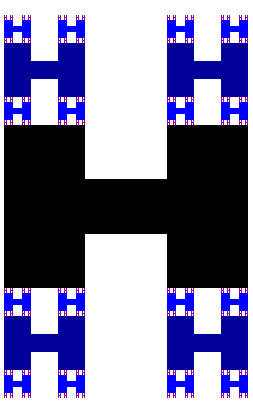
\includegraphics[max width=\textwidth]{hrcrsn}
\end{center}

Kids play with recursions. Draw a big H. Draw 4 smaller H's on the ends of the first one. Draw another 16. Then 64. Everywhere you look the picture is made of the H shape. The picture is recursive.

Some readers may recognise this as a slight elaboration of Cantor's middle-third set, in which the middle third of a line is removed, then the middle third of each of the two remaining lines is removed, and so on as shown below.

\begin{center}
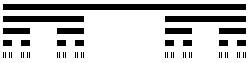
\includegraphics[max width=\textwidth]{cantorm3}
\end{center}

This particular example of a self-similar recursion occurs in numerous writings.

Other well-known examples include the Koch snowflake and the Mandelbrot set.

\section*{NESTED SETS OF RECURSIVE SYSTEMS}
The Viable Systems model is a recursive system.

Originally this was a mathematical model, but happily Beer re-thought his ideas in graphical terms. For many people this is the ideal medium, you can see the problems you are dealing with as a series of drawings, and the complex relationships can be identified within the patterns of lines and loops and arrows.

\textbf{The basis for this recursiveness is the assertion that all viable systems look the same.}

Regardless of its size, all viable organisations look like this; they have an operational part which performs the basic activities, a Metasystem which is charged with providing the services needed by the operational units so that they coheres into a greater whole, and an environment which is in constant interaction with both the operation and the Metasystem. And within these three elements the same rules for Viability can be identified.

\begin{center}
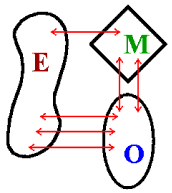
\includegraphics[max width=\textwidth]{vsmbasct}
\end{center}

\textbf{"To cybernetic eyes all viable organisations look exactly the same.
They are all underwritten by the same laws."}

\begin{center}
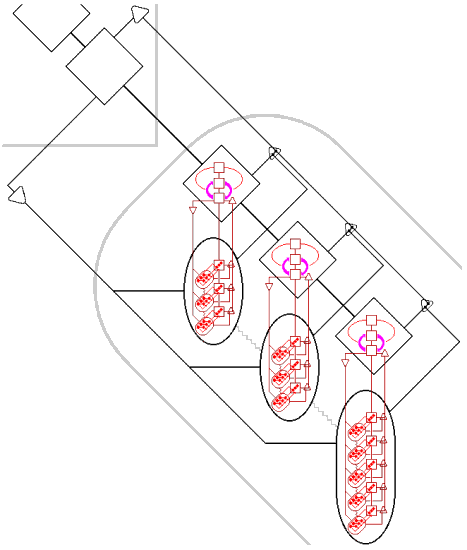
\includegraphics[max width=\textwidth]{vsm5rcsn}
\end{center}

So, if you decide to examine the working of any viable system and zoom in on the operation, you will find a series of smaller viable systems all looking exactly the same as the larger whole.

And just like the automobile investigator, if you decide to raise your perspective, you will find that the system-in-focus is itself embedded in a larger viable system.

Over the last forty years the VSM has been applied to dozens of biological systems and the fundamental recursiveness of nature becomes abundantly clear. From cells to organs to plants and animals, from beehives to oak trees to rainforests, the entire biosphere including the planet itself can best be understood as a set of nested recursive systems.

The same should be true of our businesses and communities and institutions and governments. The current work is concerned with small scale, self-managed viability. Those of you interested in the viability of governments and federations of Nation states and the United Nations are wholeheartedly encouraged to read Beer's work in dozens of publications since 1970.

\section*{FROM THEORY INTO PRACTICE}
This book is designed as a practical guide for people who actually want to use the VSM, and while all this stuff on recursions and cells being the same as the whole planet is all very entertaining, what possible use can it be to anyone concerned with solving organisational problems. Where do you begin?

\subsection*{The First point is focus}
In dealing with a problem it is crucial to identify exactly the boundaries within which the problem is found. There is no point in trying to deal with inefficiency within a particular department unless you have a clear model of the multitude of interactions which will be involved.

Once you have sketched out your organisation as a series of nested viable systems (and it may take some time to clearly disentangle all the recursions) you then have a starting point for your diagnosis.

Other (non-recursive) models don't provide this focus. Either they are concerned with who is responsible to who ... ( so where are the trucks and computers?) or they involve huge flow diagrams covering aspects of several recursive layers, and thus tend to bewilder rather than clarify.

\subsection*{The second point is the universal definition of Viability}
All the Viable systems and all their embedments at all levels throughout the known galaxy have the same structure.

They can all be diagnosed using an absolutely precise definition of Viability.

The practical advantages of this are clear: by disentangling and drawing the recursions you then have the basis for understanding every aspect of the system-in-focus, regardless of its status or size or the power it wields. To cybernetic eyes they are all exactly the same.

\textbf{Beer calls this "the parsimony of natural invariance"}

\subsection*{So where do you begin?}
First of all take pencil and paper and sketch levels of recursion. Much of what follows will involve sketches, so you should get used to dashing off quick drawings. An example is given on the next page.

\section*{DRAWING LEVELS OF RECURSION}
Imagine you have been asked to undertake the study of a large multinational company. You begin by attempting to draw an organisational chart of the whole thing. After several hours you have a several square yards of paper covered with lines and notes and scribbles which is progressively becoming more and more incomprehensible. What can you do?

\textbf{Beer sez "draw the recursions"}

\begin{itemize}
  \item \textbf{Recursion 1 - the whole corporation} sub-systems (system 1) the 3 divisions
  \item \textbf{Recursion 2 - the divisions} system 1 ... 3 companies in this one, 5 in the second
  \item \textbf{Recursion 3 - companies} containing plants
  \item \textbf{Recursion 4 - plants} containing departments
  \item \textbf{Recursion 5 - departments} containing people
\end{itemize}

(Please note: a complete diagram would require the addition of all the other circles. Three divisions, 11 companies, 53 plants and so on.)

\section*{WORKING WITH LEVELS OF RECURSION}
Once you have teased apart the levels of recursion, you can begin to diagnose. This could either be a complete study of the corporation, or as is more likely, it could be a study of a particular problem.

In both cases this involves defining carefully your system in focus. Once this is clear, you can begin to apply the procedures which define the VSM. What are the operational units? Are the four elements of the Metasystem identifiable and working properly? Are the environmental interactions OK?

But you always have to begin with complete clarity about the level of recursion. Each level consists of complete viable systems which are whole and must function (viably) as autonomous entities. If you don't have this clarity, you may try and take into account other parts of the over-all organisation which are not part of the system in focus and which therefore should not be part of this aspect of the diagnosis.

During his work in Chile, Beer projected large diagrams of the various levels of recursion within the Chilean social economy which he used to focus the attention of the people discussing a particular problem. Invariably the discussion would wander up and down the levels of recursion and Beer would say "Excuse me, but this is not part of this recursion and should be put on one side until the current discussion is concluded" (Recursion monitors may well be a crucial job for the next millennia).

The power of all of this is staggering:

\begin{itemize}
  \item As all recursions work in the same way, the tools for dealing with problems at global and international level are exactly the same as those for dealing with a bunch of kids in a youth-club. Once you have an understanding of the VSM, there's nothing to stop you redesigning the United Nations.

  \item Defining the system in focus concentrates your attention on exactly what you need to know. The other 99\% of the organisation can confidently be ignored (at this time) thus giving you a precise, limited environment in which to work. Imagine trying to decide on which part of the many yards of organisational chart you need ....

  \item Working with levels of recursion alone can bring insights. You may find that after a dozen attempts at drawing the levels that the only way to make sense of it all, is to re-think the whole thing in a new way.

\end{itemize}

\section*{CASESTUDY}

\section*{WHY DON'T LARGE GROUPS WORK?}
Take any growing democratic organisation working without authority structures. When numbers are small everything works well. At around 15, problems emerge. At about 20, these problems make it inevitable that smaller functional groupings occur. In the UK problems with organising large groups of people democratically have posed so many problems that some groups have actually shunned expansion to keep their structure small and manageable.


\section*{The VSM looks like this:}
\textbf{The crucial mechanism is thorough discussion between all members.} \textbf{Complete VSM diagnosis reveals a thoroughly workable (albeit unstructured) system.}

\section*{CASE STUDY -}

\section*{WHY DON'T LARGE GROUPS WORK?}

\subsection*{VSM diagnosis}
Look out! Another level of recursion has generated spontaneously!

People arrange themselves into small departmental groups for several reasons ...

\begin{itemize}
  \item they provide a focus for dealing with problems

  \item they get round the horrendous problems of trying to communicate with dozens of other people on a continuous basis

  \item they allow expertise to accumulate in coherent groupings

  \item they work well as teams

\end{itemize}

So how do we do a VSM diagnosis of this?

Some of the members are shown working as five teams, each of which (from the previous page) can be assumed to function as a Viable System It's inevitable that some people's jobs won't fit neatly into this strategy. Someone has to pay the bills, and keep the books. Someone has to ensure that the allocation of personnel to the various groups is handled properly to deal with sickness and holidays.

What is now essential is a look at the next level of recursion up, in which the Operational units are departments, and the job of the Metasystem is to ensure that departments work together as a coherent whole.

\section*{CASE STUDY -}

\section*{WHY DON'T LARGE GROUPS WORK?}

\subsection*{VSM diagram of the next level of recursion up}
\textit{System in focus - the organisation as whole.}

This diagram now represents the whole organisation, and within the Operation there will be five smaller identical diagrams representing the departments (\href{https://vsmg.lrc.org.uk/screen.php?page=recursion#largevsm}{have a look at the large diagram in section above})

The previous section had a brief look at the organisation of one small team and declared it viable. The current job is to look at the whole organisation, ignore the goings on inside the operational units which are not the concern of this level of recursion, and to see how it looks.

The questions are as follows:

The details of this process for Suma are covered in the next chapter - the somewhat staggering conclusion was that almost none of the Metasystemic activity was getting done, and that if the VSM was right, a series of new functions needed to be designed quickly to ensure viability.

Relating this back to the original physiology, the unstructured system had essentially no brains! And all of the problems which had emerged could be neatly allocated to one of the missing systems which Beer maintains are essential for viability.

\section*{CASE STUDY -}

\section*{WHY DON'T LARGE GROUPS WORK?}

\subsection*{Summary}
Everything which happens as a small group grows into a large group can be explained by an analysis based upon a transition from a

two recursions system (people and Business)

to

a three recursions system (people, departments and Business)

At the time this study was undertaken, most people working in the UK had blithely assumed that efficient, people-centred businesses could be built by rejecting hierarchy and basing effective organisation on highly motivated self-managed individuals. The structure would only involve regular meetings and some specialisation. Everything else would take care of itself. Everyone knew it worked for small groups, and it was assumed that it could be extended to a large organisation.

The reality was very different. A paper by an American feminist called "The Tyranny of Structurelessness" argued that in large groups, the lack of structure guaranteed that many individuals would be ignored and that people with dominant personalities would flourish. It became clear that one of the sacred cows of co-operative working had to be slaughtered, and that the kind of egalitarian working practices which were central to our vision could only be ensured through a carefully designed structure.

So the answer to the question is:

\begin{itemize}
  \item It's impossible to involve more than about 7 people in an effective and unstructured organisation because of the practicalities of communication.

  \item Organisations break into small teams, because they work.

  \item This means an extra level of recursion introduces itself.

  \item The business becomes an entirely different animal. Each work team has to work as a viable system in its own right, and a series of new functions become essential as the departments themselves need the services of a Metasystem.

\end{itemize}

Before undertaking this study no-one had suspected that grouping into departments would have any consequences. We work in teams. ... so what?

Thankfully the VSM lays down the rules for dealing with this, and this is developed in the next chapter.
